\newpage
\section{Alarm og feilhandtering}
\thispagestyle{fancy}

% Skriver litt om introduksjon om alarm og feilhandtering
Alarm og feilhandtering utgjer ein sentral del av eit velfungerande styresystem. Det er avgjerande
at anlegget effektivt handterer og varslar om uønska hendingar, slik at 
driftspersonell blir varsla og naudsynte tiltak kan utførast. \nocite{Olav}

% Skrive litt om codesys alarmhantering
For å varsle om alarm og feil har vi nytta oss av \gls{Codesys} sine
innebygde alarmhandteringsfunksjonar \citep{CodesysAlarm}. Desse funksjonane gir oss høve til å 
kontrollere, gruppere og prioritere alarmar, samt å sende informasjon til driftspersonell.

% Skriver om alarmar både gamle og nye.
\gls{IEC}-blokkene gir oss moglegheit til å detektere ulike typar hendingar som feil, alarm og forvarsel.
Dei forskjellige blokkene har ein ulik mengde hendingar som skal kunne detekterast og varslast.
Alle desse moglege varslingane er samla i programmet saman med dei aktive varslingane som er i bruk på Sande reinseanlegg i dag. (Vedlegg E)

Vi har valt å dele opp alle varslingane i fire forskjellige grupper:

\begin{itemize}
    \item \textbf{Feil}          (Der system ikkje fungerer, t.d. sensorfeil og blokkfeil)
    \item \textbf{Alarm}         (Kritiske prosessparametrar, t.d. straumbrot og veldig høge nivå)
    \item \textbf{Forvarsel}     (Prosessparametrar nærmar seg kritisk nivå)
    \item \textbf{Informasjon}   (Prosessinformasjon med nytteverdi)
\end{itemize}

Ved å kategorisere varslingar i fire ulike grupper med forskjellige prioriteringsnivå,
vil system og driftspersonell enklare kunne forstå samanhengen og alvoret i varslingane. \newline
Korleis dei ulike alarmane blir definert og prioriterte må evaluerast i samråd med \gls{Sunnfjord Kommune}.

\begin{figure}[htbp]
    \centering
    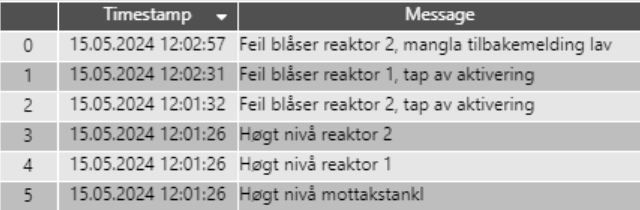
\includegraphics[width=0.6\textwidth]{Bilder/Alarmeksempel.png}
    \caption{Varslingar implementert i simulering}\label{fig:Alarmlogg}
\end{figure}

\newpage

